%%%%%%%
% Ch4 %
%%%%%%%

\setcounter{chapter}{3}
\chapter{Ponts universels}
	\begin{wrapfigure}[5]{l}{6 cm}
	\vspace{-5mm}
	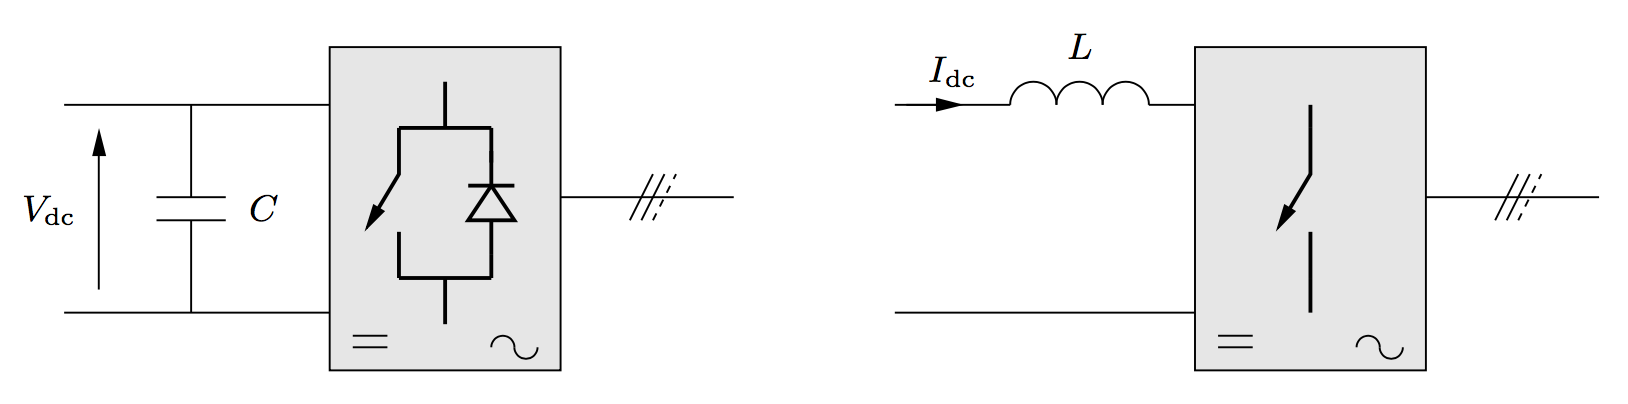
\includegraphics[scale=0.2]{ch4/1}
	\captionof{figure}{}
	\end{wrapfigure}
	Les \textbf{onduleurs autonomes} possèdent généralement une structure en pont et sont constitués d'intérupteurs commandables. Ils peuvent être alimenté par une source de tension continue (voltage source converter, VSC) ou par une source de tension continue (CSC), les deux modèles différents par un condensateur ou une inductance dans le bus d'entrée. Ils peuvent fonctionner en \textbf{redresseur}. Les hacheurs \textbf{multi-quadrants} utilisé entre autre pour la commande de moteur à courant continu ont la même topologie avec une commande semblable. 
	
	\begin{minipage}{0.5\textwidth}
		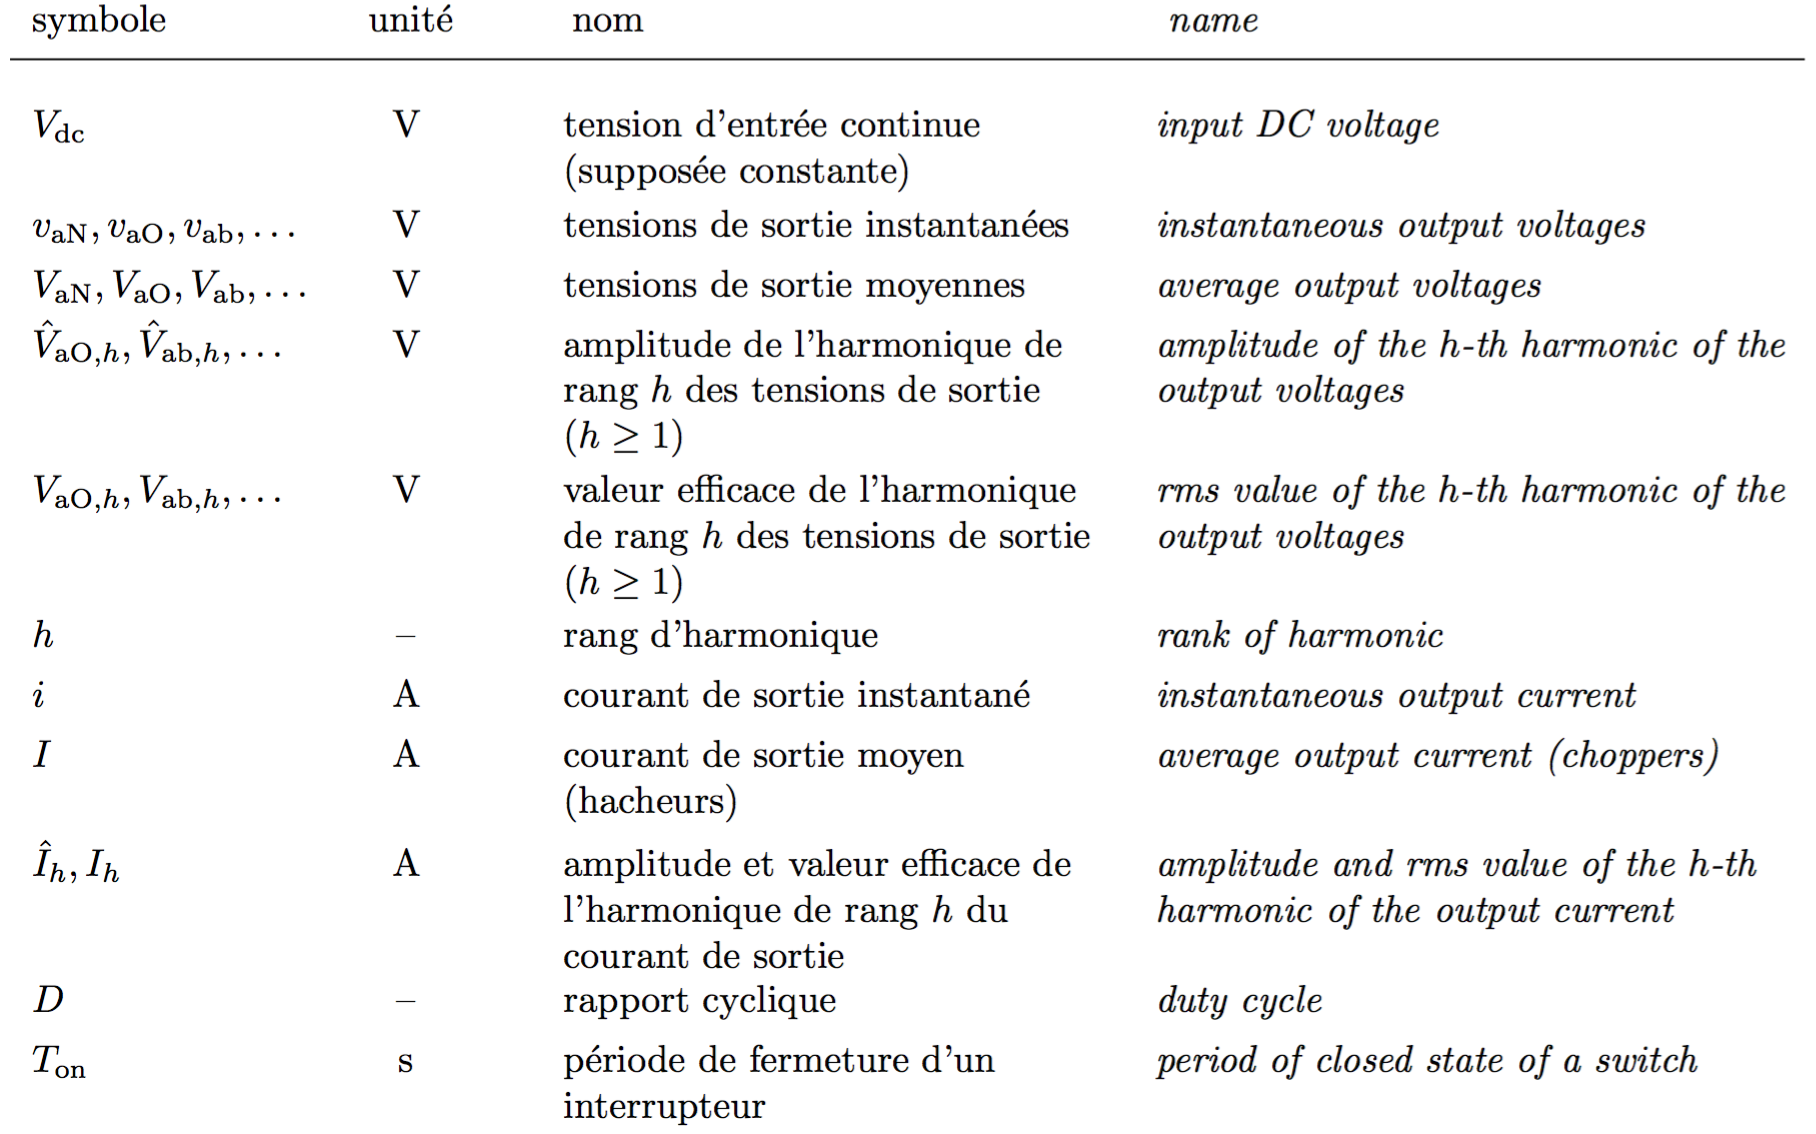
\includegraphics[scale=0.25]{ch4/2}
	\end{minipage}
	\begin{minipage}{0.5\textwidth}
		\vspace{3mm}
		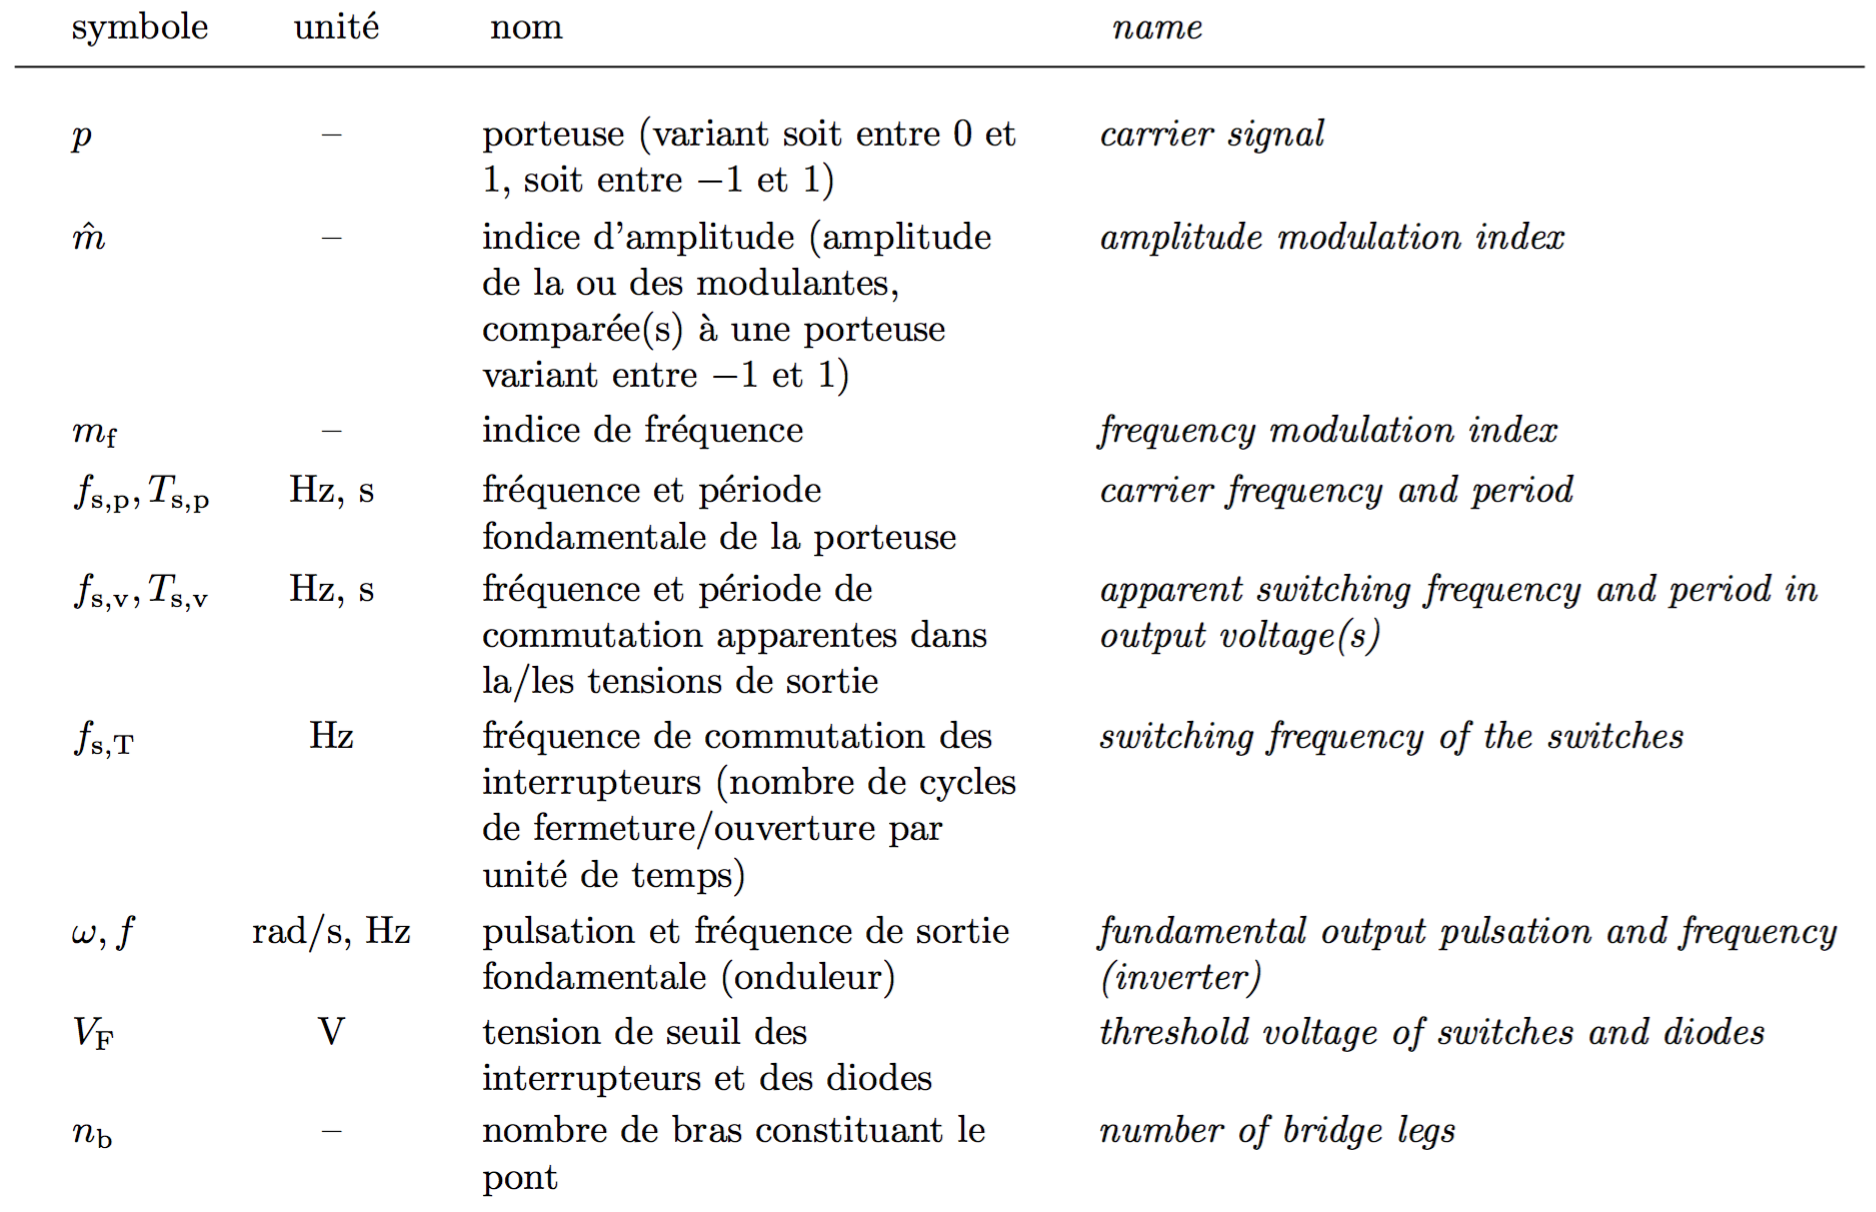
\includegraphics[scale=0.25]{ch4/3}	
	\end{minipage}
	\captionof{table}{Liste des abréviations et symboles.}
	
\section{Caractéristiques des interrupteurs commandables}
	\begin{wrapfigure}[4]{r}{5 cm}
	\vspace{-5mm}
	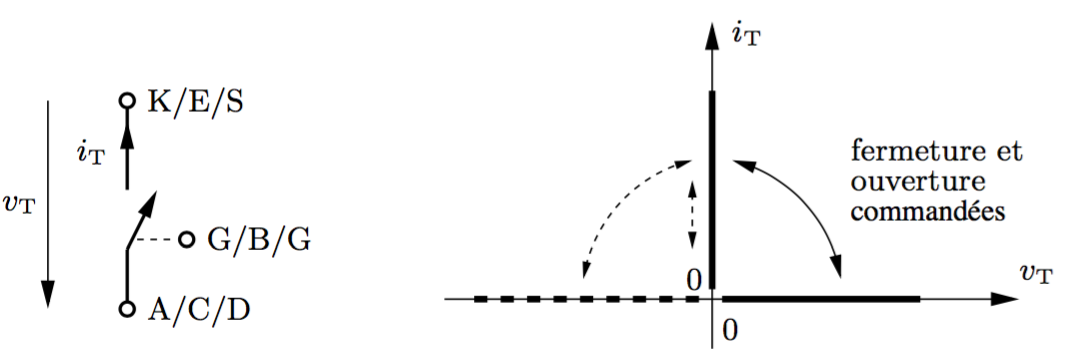
\includegraphics[scale=0.25]{ch4/4}
	\captionof{figure}{}
	\end{wrapfigure}
	Ci-contre, la caractéristique tension-courant idéalisée d'un interrupteur commandable. Le 2${ème}$ quadran ne nous intéresse pas puisque la tension $v_T$ y est négative et est exclue lorsqu'une diode est raccordé en anti-parallèle sur l'interrupteur. \\
	
	\begin{wrapfigure}[6]{l}{6 cm}
	\vspace{-5mm}
	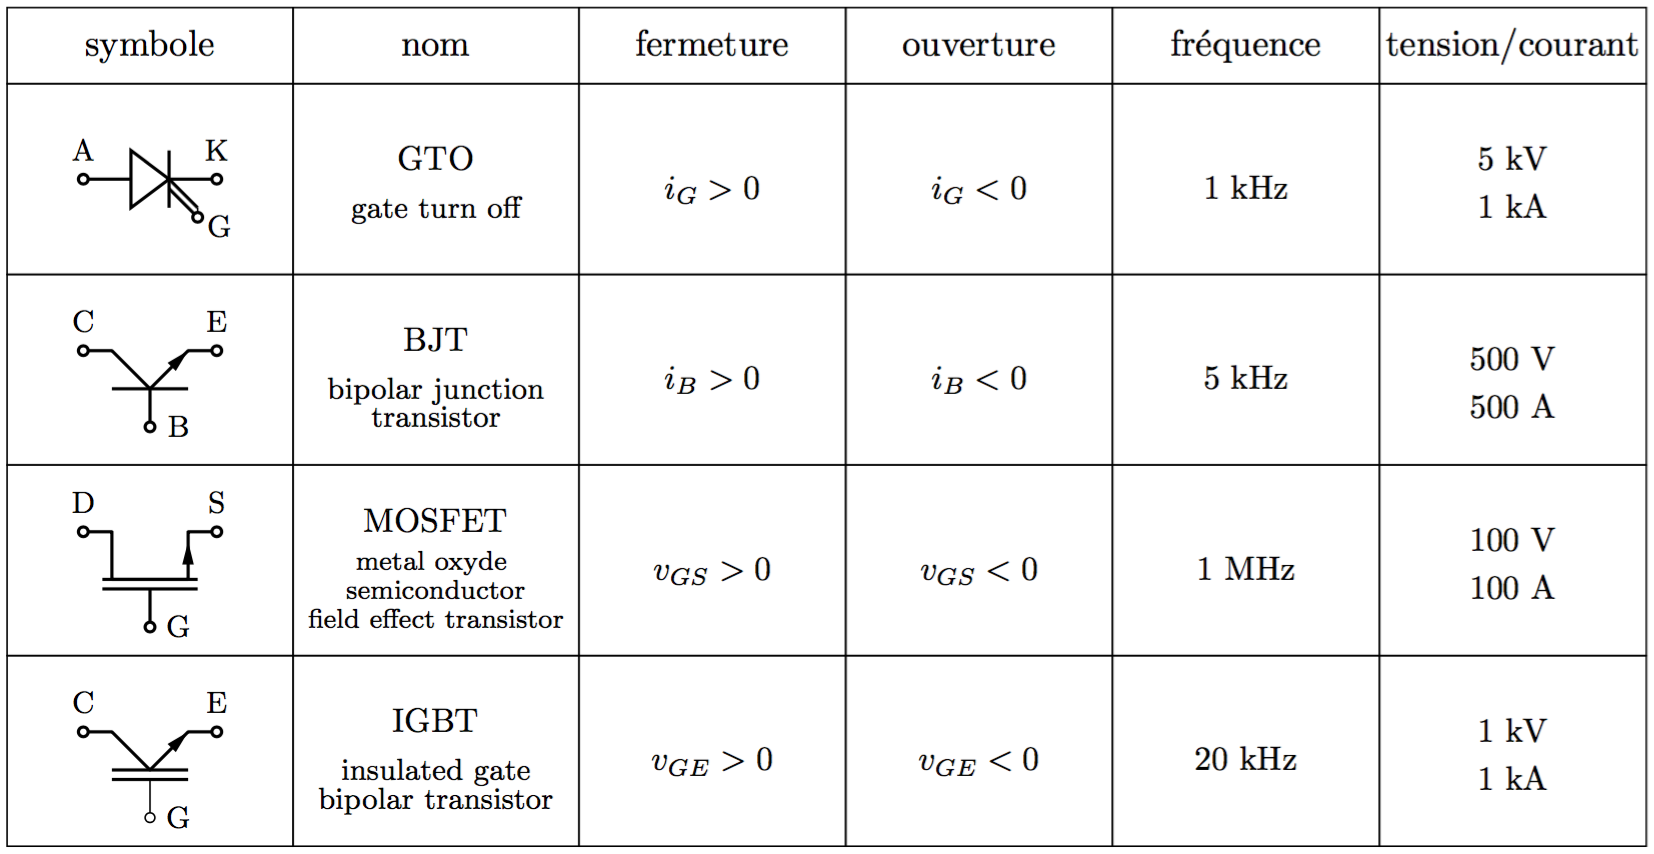
\includegraphics[scale=0.2]{ch4/5}
	\captionof{figure}{}
	\end{wrapfigure}
	Ils sont tous \textbf{unidirectionnnels} donc le courant ne peut circuler que de l'anode A vers la cathode K, du collecteur C vers l'émetteur E ou du drain D vers la source S. L'\textbf{électrode de commande} (gachette G, base B ou grille G) permet d'effectuer la fermeture et ouverture de l'interrupteur grâce à une tension ou un courant. 
	
	La tension $V_{T,max}$ et le courant $I_{T,max}$ maximum supportée ou conduit par l'interrupteur sont limités. On peut faire des montages en série ou parallèle pour augmenter la puissance nominale mais il va falloir faire une répartition uniforme du courant et tension. La commutation entre l'état passant et bloqué prend un certain temps plus ou moins important, ce qui limite la fréquence de commutation $f_{s,T}$. Durant ces intervalles, la tension et le courant sont tout deux importants et donnent lieu à des \textbf{pertes de commutation}.
	
\section{Convertisseurs à source de tension : généralités}
\section{Hacheurs - modulation de largeur d'impulsions (MLI)}
	 \textbf{Pulse with modulation (PWM)} est une des méthode de commande des bras du convertisseur. La fréquence de commutation est maintenue constante et pour chaque bras, la période de commutation est scindée en 2 partie où c'est d'abord l'interrupteur supérieur qui est fermé puis l'inférieur. En modulant la durée des sous-intervalle, on génère la tension moyenne. \\
	 Les tensions sont entachés d'une série d'harmoniques en raison de la commutation. Les charges inductives font que les courants sont en meilleur état. Notons qu'en cas de commande à hystérésis, la fréquence de commutation n'est pas constante et ce pour les harmoniques aussi (filtres). \\
	 La \textbf{MLI intersective} consiste à déterminer les instants de commutation pour un bras en comparant la \textbf{porteuse p(t)}, signal triangulaire de fréquence $f_{s,p}$ et la \textbf{modulante}, image de la tension souhaitée. Pour les ponts en H dans le cas monophasé, il est possible d'utiliser la même modulante pour les 2 bras (modulation bipolaire) ou d'en prendre 2 séparés (modulation unipolaire). Pour un pont onduleur/redresseur \textbf{triphasé} il faut considérer trois modulantes formant un système triphasé équilibré. \\
	 Lorsque la commande est faite avec de l'électronique analogique, la comparaison de p(t) et m(t) est fait telle quelle. Avec de l'électronique digitale, même résultat obtenu sans réelle comparaison (rapport cyclique). 
	 
	 \subsection{Demi-pont}
	 	\subsubsection{Sans point milieu à l'entrée}
	 		\begin{wrapfigure}[8]{l}{6.5cm}
			\vspace{-5mm}
			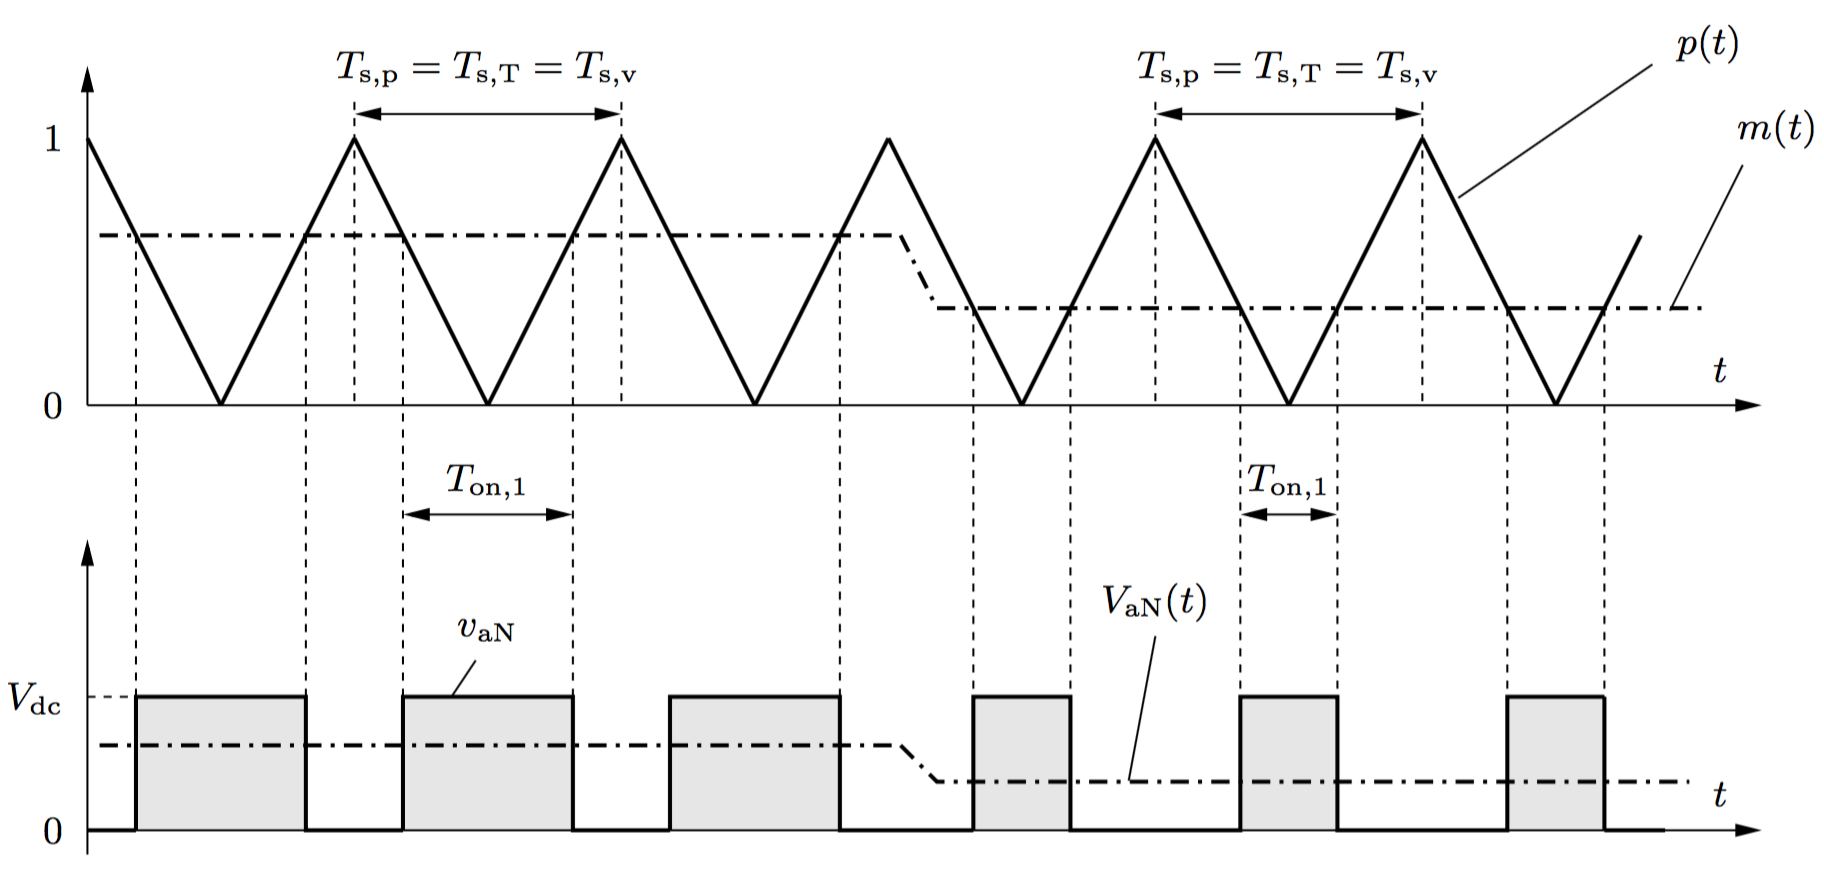
\includegraphics[scale=0.2]{ch4/6}
			\captionof{figure}{}
			\end{wrapfigure}
			Comme la tension de sortie $v_{aN}(t)$ est toujours positive ou nulle, on prend p(t) triangulaire variant entre 0 et 1. La m(t) est supposée varier lentement (constante sur une période de commutation $T_{s,p}$) par rapport à la porteuse. Quand $m(t) > p(t)$, l'interrupteur supérieur du bras est fermé et $v_{aN} = V_{dc}$. Quand $m(t) < p(t)$, c'est l'interrupteur inférieur qui est fermé et $v_{aN}$ = 0. On suppose que la m(t) est aussi comprise entre 0 et 1.  